\documentclass[
	a4paper,     		%% Papiergroesse: A4 OBSOLETE
%	twoside,     		%% Zweiseitiges Layout (alternativ: oneside)
	headsepline, 		%% Horizontale Linie unter Kopfzeile
	footsepline, 		%% Horizontale Linie ueber Fusszeile
	titlepage,   		%% Eigenstaendige Titelseite (alternativ: notitlepage)
%	halfparskip, 		%% Halbe Leerzeile zwischen zwei Abschnitten (alternativ: parskip, ...)
%	12pt,        		%% Schriftgroesse: 12pt (alternativ: 10pt, 11pt, ...) OBSOLETE
%	bibtotoc,			%% Bilbiographie in's Inhaltsverzeichnis aufnehmen
%	liststotoc,			%% Indexe in's Inhaltsverzeichnis aufnehmen
%	smallheadings,		%% Kleine Ueberschriften
%	DIV1,				%% Divisor, Zeilenlänge ca. 70 Zeichen
%	BCOR01cm,			%% Bindekorrektur
%	draft			  	%% Entwurfsmodus, volle/leere Boxen markieren
%	abstracton			%% Titel "`Zusammenfassung"' einschalten
]{scrreprt}

%%%
%%% Pakete
%%%

%%% Glossar
% \usepackage[german]{gloss}
% \newcommand{\acr}[1]{{\small\gloss[word]{#1}}}
% 
% \newcommand{\abk}[1]{#1\xdot}
% \DeclareRobustCommand\xdot{\futurelet\token\Xdot}
% \def\Xdot{\ifx\token\bgroup.\else\ifx\token\egroup.\else
%   \ifx\token\/.\else\ifx\token\ .\else\ifx\token!.\else
%   \ifx\token,.\else\ifx\token:.\else\ifx\token;.\else
%   \ifx\token?.\else\ifx\token/.\else\ifx\token'.\else
%   \ifx\token).\else\ifx\token-.\else\ifx\token+.\else
%   \ifx\token~.\else
%   \ifx\token.\else.\ \fi\fi\fi\fi\fi\fi\fi\fi\fi\fi\fi\fi\fi\fi\fi\fi} 
% \newcommand{\zB}{\mbox{z.\,B}\xdot}

%%% Literaturverzeichnis, deutschen Stil benutzen (dinat)
%%% TODO: funktioniert leider derzeit nicht mit TeXlipse!
%\usepackage[square]{natbib}
%\citestyle{dinat}

%%% Grafik
\usepackage{pstricks}

%%% Subfigures
\usepackage{subfig}

%%% UML
%\usepackage{pst-node}
%\usepackage{pst-uml}
%\let\umlClass\pstumlClass	%%% workaround: pst-uml und uml kollidieren
%\usepackage{uml}

%%% Deutsche Sprache verwenden
\usepackage{ngerman}

%%% Kodierung der Eingabezeichen setzen (fuer dt. Umlaute etc.)
%%% Für Linux: [latin1] für Windows: [ansinew]
\usepackage[utf8]{inputenc}

%%% Zeichen-Kodierung in PDF-Dokumenten
\usepackage[T1]{fontenc}
%\usepackage{ae,aecompl}

%%% Web-Addressen auch mit T1-Encoding
\usepackage[T1]{url}
%%% ... und in tt-Font
\urlstyle{tt}

%%% amsmath, amssymb, amstext: Unterstuetzung div. mathematischer Zeichen etc.
\usepackage{amsmath,amssymb,amstext}

%%% pifont: "pifont Xs and Check Marks"
% \usepackage{pifont}

%%% PostScript-Fonts ersetzen
\usepackage{psfrag}

%%% Programmcode einbinden, Listings
\usepackage{listings}

%%% Farb-Unterstuetzung
\usepackage{color}

%%% Tabellen
\usepackage{booktabs}
\usepackage{array}
\usepackage{multirow}
\usepackage{tabularx}
\usepackage{threeparttable}	% Fussnoten in table-Umgebung

%%% Floats strikter positionieren (Option 'H'ere)
\usepackage{float}

%%%
%%% Pakete konfigurieren, Definitionen
%%%

%%% Ueberschriften bis zur Ebene 3 nummerieren
\setcounter{secnumdepth}{3}
\setcounter{tocdepth}{3}

%%% Neue Spaltentypen definieren
\newcolumntype{N}{>{\bfseries\scriptsize}l}
\newcolumntype{V}[1]{
	>{\bfseries\scriptsize\raggedright\hspace{0pt}}p{#1}
}

%%% Ein paar Farbdefinitionen (s. http://texnik.de/listings/listing0.pdf)
\definecolor{hellgelb}{rgb}{1,1,0.8}
\definecolor{hellgrau}{rgb}{0.95,0.95,0.95}
\definecolor{colKeys}{rgb}{0,0,1}
\definecolor{colIdentifier}{rgb}{0,0,0}
\definecolor{colComments}{rgb}{1,0,0}
\definecolor{colString}{rgb}{0,0.5,0}

%%% Konfiguration des listing-Paketes
\lstset{%
	%float=hbp,%
	%basicstyle=\ttfamily\footnotesize, %
	identifierstyle=\color{colIdentifier}, %
	basicstyle=\ttfamily\small,%
	stringstyle=\ttfamily,%
	keywordstyle=\color{colKeys}, %
	stringstyle=\color{colString}, %
	commentstyle=\color{colComments}, %
	columns=flexible, %
	tabsize=2, %
	frame=tb, %
	extendedchars=true, %
	showspaces=false, %
	showstringspaces=false, %
	numbers=left, %
	numberstyle=\tiny, %
	breaklines=true, %
	backgroundcolor=\color{hellgelb}, %
	breakautoindent=true, %
	captionpos=b%,
	aboveskip=\bigskipamount,%
	belowskip=\medskipamount,%
	escapeinside={(*}{*)}, %
	mathescape = true, %
	language=Matlab, %
}

%%% Benoetigte Sprachen laden
\lstloadlanguages{Matlab}

%%%
%%% Seitenlayout, Schriften
%%%

%%% scrpage2: KOMA Kopf- und Fusszeile
\usepackage[automark]{scrpage2}

%%% KOMA-Script: Optionen
% \KOMAoptions{fontsize=12pt}
% \KOMAoptions{paper=a4}

%%% EM unterstrichen darstellen
%\usepackage{ulem}

%%% Schrift fuer Captions verkleinern
\setkomafont{captionlabel}{\scriptsize}
\setkomafont{caption}{\usekomafont{captionlabel}}

%%% Schrift fuer Ueberschriften umstellen
%\setkomafont{sectioning}{\normalcolor\bfseries}

%%% Schriften fuer Titel- und Fusszeile umstellen
%\setkomafont{pagehead}{\normalfont\sffamily}
%\setkomafont{pagenumber}{\normalfont\rmfamily\slshape}

%%% Unterstuetzung fuer Grafiken
\usepackage[dvips]{graphicx}
\DeclareGraphicsExtensions{.eps}
\graphicspath{{../images}}

\makeatletter
\renewcommand{\fps@figure}{htbp}
\renewcommand{\fps@table}{htbp}
\makeatother

%%% Hyperlinks in PS-Dokumenten, Optionen s.o.
\usepackage[%
  dvips,%
  colorlinks=false,%
  breaklinks=true,%
]{hyperref}

%%% Informationen ueber das PDF-Dokument setzen
\hypersetup{
  pdftitle={Aufgabe 1 - Schilddrüsenfunktion},%
  pdfauthor={Jan Tammen (jan.tammen@htwg-konstanz.de)},%
  pdfsubject={Neuronale Netze und Fuzzy-Logik},%
  pdfcreator={Jan Tammen (jan.tammen@htwg-konstanz.de)},%
  pdfkeywords={Aufgabe 1, Schilddrüsenfunktion},
  pdfproducer={\LaTeX\ with package \flqq hyperref\frqq}, %%
  colorlinks=true,
%  linkcolor=Gray,
%  urlcolor=Gray,
  bookmarksopen=true,
  pdfpagemode=UseOutlines,
  pdfview=FitV, % FitH
  pdfstartview=FitV,
  pdfhighlight=/I,
%   pdfborder=0 0 0, % keine Box um die Links!
  bookmarksnumbered=false,
  plainpages=false,
}

%%% Links im dvips-Mode auch umbrechen
%\usepackage{breakurl}

%%%
%%% Layout der Titelseite
%%%

%%% Titelkopf, erscheint oberhalb des Titels
\titlehead{
	\begin{figure}[H]
		\centering
		
\includegraphics[width=\textwidth]{../images/htwg-logo}
	\end{figure}
}

%%%% Subject, erscheint oberhalb des Titels
\subject{Neuronale Netze und Fuzzy-Logik, SS 07}

%%% Titel
\title{Aufgabe 1 - Schilddrüsenfunktion}


%%% Publisher, hier: Verantwortlicher Prof.
\publishers{%
	\small
  Prof.\ Dr.\,Bittel, HTWG Konstanz
}

%%%% Autor. Weitere Autoren mit \and{<Name>} hinzufuegen
\author{%
	Jan Tammen, Matrikel-Nr. 277143
}%

%%% Datum setzen
\date{4.\ Juli 2007}

%%% Rueckseite der Titelseite
\lowertitleback{%
	\footnotesize%
	Erstellt mit \LaTeXe\ unter Verwendung des \KOMAScript-Pakets.
}

%%%
%%% Header und Footer
%%%

\pagestyle{scrheadings}

%%% Kopfzeile in den Rand ragen lassen
%\setheadwidth{textwithmarginpar}

%%% Fusszeile in den Rand ragen lassen
%\setfootwidth{head}

%%% \automark[rechte Seite]{linke Seite}
%\automark[subsection]{section}

%% Header links -- section
%\ihead[]{\rightmark}

%% Header rechts -- chapter
%\ohead[]{\leftmark}

%% Header mittig -- leer
\chead[]{}

%% Footer mittig -- leer
\cfoot[]{}

%% Footer rechts -- Seitenzahl
\ofoot[]{\thepage}

%%% Footer links -- Titel der Arbeit
\ifoot[]{\footnotesize{Aufgabe 1 - Schilddrüsenfunktion}}

%%%
%%% Sonstiges
%%%

%%% Glossar und Index erstellen 
% \makegloss
% \makeindex

%%%
%%% Beginn Hauptdokument
%%%
\begin{document}

%%% Titelseite erstellen
\maketitle

%%% Inhaltsverzeichnis erstellen
%\newpage
\tableofcontents

%%% Bildverzeichnis erstellen
%\newpage
%\listoffigures

%%% Tabellenverzeichnis erstellen
%\newpage
%\listoftables

%%%
%%% Beginn Inhalt
%%%
\chapter{Beschreibung der Aufgabenstellung}
Es soll ein neuronales Netz entworfen werden, welches in der Lage ist zu
entscheiden, ob bei einem Patienten eine Fehlfunktion der Schilddrüse vorliegt.
Dazu müssen die Werte 21 verschiedener Attribute ausgewertet werden. Anhand der
hohen Anzahl der Attribute lässt sich erkennen, dass eine solche
\emph{Klassifizierungsaufgabe} mit herkömmlichen Methoden eher schwierig lösbar
wäre. Daher wird hier auf die Verwendung eines künstlichen neuronalen Netzes
zurückgegriffen, welche sich gut zur Klassifikation und Mustererkennung nutzen
lassen.

In der vorliegenden Arbeit sollen zunächst die zur Verfügung stehenden Daten
analysiert, in Test- und Trainingsdaten aufgeteilt und anschließend ein
entsprechendes neuronales Netz mithilfe der \emph{Neural Networks Toolbox} der
Mathematiksoftware Matlab implementiert werden. Ziel ist es, eine
Klassifizierungsrate zu erreichen, die deutlich über 92\% liegt.



\chapter{Lösungsansatz}
\section{Analyse und Aufbereitung der Daten}
Die vorliegende Datei \texttt{thyroid.dat} enthält die Datensätze von 7200
Patienten und soll als Basis für das Training und den Test des zu erstellenden
neuronalen Netzes dienen. Ein Datensatz enthält dabei jeweils 21 verschiedene
Attribute, 15 davon in binärer Form und 6 reellwertig. Folgender Auszug aus der
Datei zeigt den Aufbau der Datensätze: 

\lstinputlisting[firstline=1, lastline=5, caption={Auszug aus der Datei
\texttt{thyroid.dat}}, label={lst:thyroid-auszug}, basicstyle=\footnotesize]{../thyroid.dat}

Es ist hier nicht bekannt, welche Attribute welchen Messwerten entsprechen - 
dieses Wissen wird für die Lösung der Aufgabe auch nicht benötigt. Wie bereits 
eingangs erwähnt, stellt die hohe Anzahl von Attributen eine erste 
Schwierigkeit dar. Weiterhin bereiten die extrem ungleich verteilten Klassen 
Probleme für herkömmliche statistische Methoden. Die letzte Spalte eines Datensatz
enthält dabei die zum Datensatz gehörige Klasse, derer es insgesamt drei gibt:

\begin{itemize}
  \item 1: "`hypothyroid"' (Schilddrüsenunterfunktion),
  \item 2: "`hyperthyroid"' (Schilddrüsenüberfunktion),
  \item 3: "`normal"' (normale Schilddrüsenfunktion).
\end{itemize}

Um zunächst einen groben Überblick über die Daten zu erhalten, wird zunächst die
Verteilung der Datensätze auf die einzelnen Klassen untersucht. Die Situation
stellt sich wie in Tabelle \ref{tbl:klassen-verteilung} aufgezeigt dar.

\begin{table}
	\sffamily
	\centering
	\footnotesize
	\begin{tabular}{lll}
		\toprule
		\multicolumn{1}{@{}N}{Klasse Nr.} &
		\multicolumn{1}{@{}N}{Anzahl} &
		\multicolumn{1}{@{}N}{Anteil [\%]} \\
		\midrule\addlinespace
		
		1 & 166 & 2,3\\
		2 & 368 & 5,1\\
		3 & 6666 & 92,6\\
		
		\addlinespace\bottomrule
		\end{tabular}

  \label{tbl:klassen-verteilung}
\caption{Verteilung der Datensätze auf die drei Klassen} 
\end{table}

\subsection{Aufteilung der Daten in Trainings- und Testdaten}
Üblicherweise werden die verfügbaren Daten zufällig aufgeteilt in eine 
Trainings- und eine Testdatenmenge. Mithilfe der Trainingsmenge wird das 
neuronale Netz erstellt und trainiert. Die Testdatenmenge dient dazu, die 
Qualität des Netzes (in Bezug auf die Vorhersagefähigkeiten) abschließend zu 
überprüfen. Es muss doch gerade in dieser Aufgabe darauf geachtet werden, dass 
die Aufteilung der Daten korrekt erfolgt. Denn betrachtet man die Verteilung 
der Datensätze auf die einzelnen Klassen, so erkennt man, dass in der Klasse 3 
die weitaus meisten Datensätze vorhanden sind (s. auch Abbildung 
\ref{fig:klassen-verteilung}). Würde man nun die Daten blindlings zufällig 
aufteilen, so erhielte man mit großer Wahrscheinlichkeit verfälschte 
Ergebnisse, da ja die meisten Datensätze in der Klasse 3 lägen. Daher wird hier 
so vorgegangen, dass die Daten zunächst in die Klassen aufgeteilt werden und 
anschließend aus jeder dieser drei Untermengen ein gleicher Prozentsatz an Datensätzen 
in den Trainigsdatenpool übernommen wird. Die verbleibenden Daten werden 
anschließend zur Simulation des Netzes benutzt, um 
dessen Generalisierungsfähigkeit zu ermitteln.

\begin{figure}
  \centering
  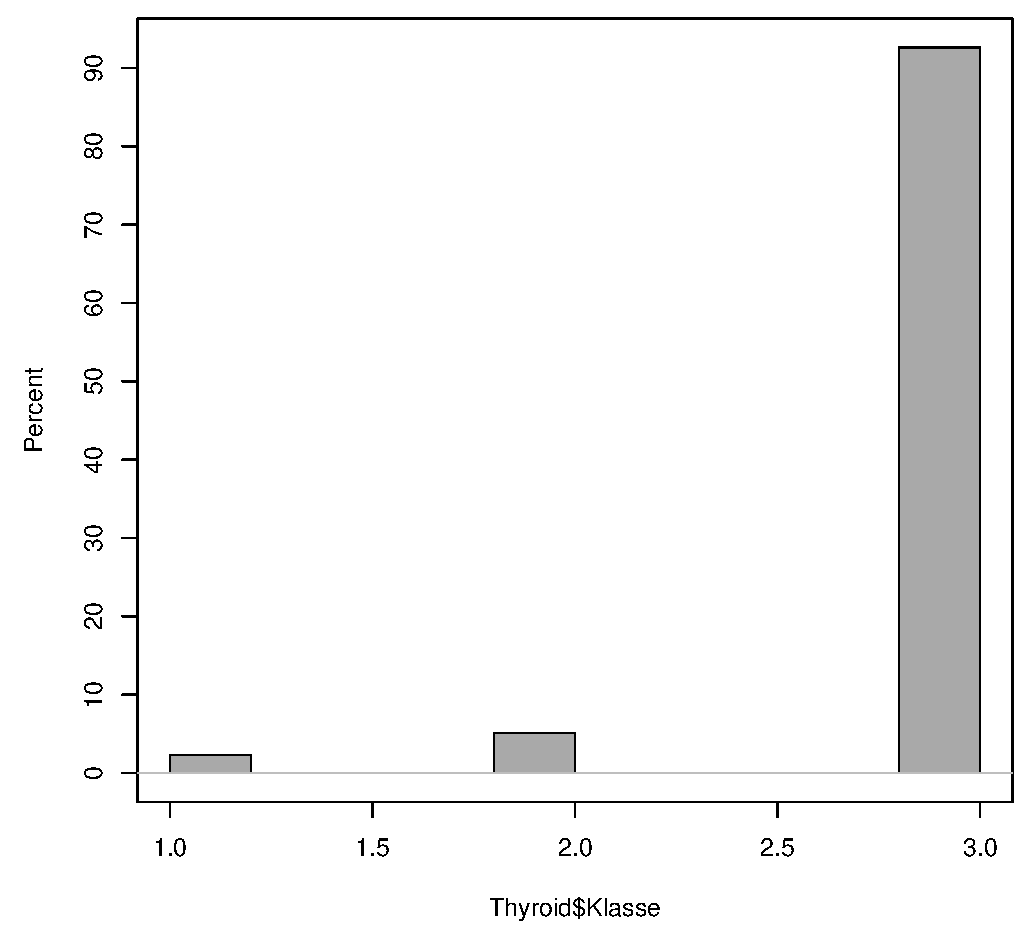
\includegraphics[width=0.6\textwidth]{../images/klassen-verteilung}
  \caption{Häufigkeitsverteilung der Klassen}
  \label{fig:klassen-verteilung}
\end{figure}

\section{Entwurf eines neuronalen Netzes}
Für die folgenden Versuche wird ein künstliches neuronales Netz vom Typ
\emph{feed-forward backpropagation} verwendet. Auf die Funktionsweise eines
Feed-Forward-Netzes wird hier nicht näher eingegangen; diese ist u.a. 
beschrieben in \cite{Demuth1998}. Erzeugt wird ein solches Netz mithilfe der 
Neural Network Toolbox in Matlab über den folgenden Funktionsaufruf:

\begin{lstlisting}[numbers=none]
[net, tr, yTrain, eTrain] = newff($PR$, [$S_1$ $S_2$ ... $S_N$], {$TF_1$ $TF_2$ ... $TF_N$}, $BTF$, $BLF$, $PF$)
\end{lstlisting}

Den einzelnen Parametern kommt dabei die folgende Bedeutung zu:

\begin{description}
  \item[$PR$] Eine $R \times 2$ Matrix mit den Minimal- und Maximalwerten der
  $R$ Eingabewerte in der Input-Schicht.
  \item[$S_i$] Größe der $i$-ten Schicht bei insgesamt $N$ Schichten.
  \item[$TF_i$] Aktivierungsfunktion der $i$-ten Schicht, Default: \texttt{tansig}. 
  \item[$BTF$] Trainingsfunktion, Default: \texttt{traingdx}.
  \item[$BLF$] Gewichts-/Schwellwertlernfunktion, Default: \texttt{learngdm}.
  \item[$PF$] Performancefunktion, Default: \texttt{mse}.
\end{description}

Für den Aufbau des Netzes wird zunächst eine \textbf{Eingabeschicht} benötigt, 
in der sich in diesem Falle 21 Neuronen befinden - eines für jedes 
auszuwertende Attribut. Die Anzahl der \textbf{verdeckten Schichten} wird 
zunächst auf 1 festgelegt. In dieser verdeckten Schicht werden 5 Neuronen
eingesetzt. Die Anzahl der Neuronen und der verdeckten Schichten wird in
weiteren Versuchen variiert werden, um eine möglichst optimale Konfiguration zu
finden (s. Listing \ref{tbl:var-neuronen} im Anhang). Für die 
\textbf{Ausgabeschicht} schließlich werden drei binäre Neuronen verwendet. Die 
Werte der einzelnen Neuronen sind dabei entweder 0 oder 1, je nach gewünschter 
Klasse:

\begin{itemize}
  \item Klasse 1: 1-0-0
  \item Klasse 2: 0-1-0
  \item Klasse 3: 0-0-1
\end{itemize} 

\subsection{Trainingsverfahren und -parameter}
Für das initiale Training des Netzes werden die folgenden Trainingsparameter
verwendet\footnote{Nicht aufgeführte Parameter wurden in der Standardeinstellung
belassen}: 

\begin{itemize}
  \item Prozentsatz von Trainingsdaten aus jeder Klasse: 10. Insgesamt 794 
  Datensätze, davon 17 aus Klasse 1, 37 aus Klasse 2 und 667 aus Klasse 3.
  \item Maximale Anzahl Epochen: 2000.
  \item Aktivierungsfunktion $TF_1$: \texttt{logsig}, $TF_2$: \texttt{logsig}.
  \item Trainingsfunktion $BTF$: \texttt{trainrp}.
  \item Performancefunktion $PF$: \texttt{mse}.
  \item Fehlerziel (\texttt{trainParam.goal}): 0.0001.
\end{itemize}

Als Trainingsfunktion wird hier die \textsl{Resilient Backpropagation}-Methode 
eingesetzt, da es nach \cite{Demuth1998} am besten geeignet ist für 
Klassifizierungsaufgaben und auch sehr performant ist. Als Fehlerziel wird MSE =
0.0001 verwendet. Bei MSE handelt es sich um den \emph{Mean Sum Squared Error}
und dieser ist definiert wie folgt: \cite[Kapitel 5]{bittel2007}.

\[
MSE = \frac{1}{N} \sum_{(p,\,t) \in L} (t_i - y_i)^2
\]

In den nachfolgenden Abschnitten sind die Ergebnisse der Testläufe mit der 
initialen Konfiguration sowie Versuche mit variierenden Netzkonfigurationen 
beschrieben.


\chapter{Ergebnisse}
\section{Testläufe mit initialer Konfiguration}
Ziel dieser ersten Testläufe war es, herauszufinden, inwieweit das Fehlerziel 
mit den gewählten Parametern erreicht werden kann. Es wurden dabei jeweils 10 
Testläufe mit identischen Parametern durchgeführt, um "`Zufallstreffer"' 
(Gewichts- und Biaswerte werden bei Initialisierung des Netzes zufällig 
vergeben) auszuschließen. Tabelle \ref{tbl:21-5-3-ergebnisse} zeigt einen
Überblick über diesen Testlauf.

\begin{table}
	\sffamily
	\centering
	\footnotesize
	\begin{tabular}{Nllc}
		\toprule
		\multicolumn{1}{@{}N}{Nr.} &
		\multicolumn{1}{V{3.5em}@{}}{Epoche} &
		\multicolumn{1}{V{3.5em}@{}}{MSE} &
		\multicolumn{1}{V{5em}@{}}{Ziel erreicht} \\
		\midrule\addlinespace

		1 & 781 & 3.239147e-003 & --- \\ \cmidrule(rl){1-4}
		2 & 268 & 3.237180e-003 & --- \\ \cmidrule(rl){1-4}
		3 & 2000 & 1.390480e-003 & --- \\ \cmidrule(rl){1-4}
		4 & 887 & 2.027749e-002 & --- \\ \cmidrule(rl){1-4}
		5 & 2000 & 1.708763e-003 & --- \\ \cmidrule(rl){1-4}
		6 & 664 & 1.756893e-002 & --- \\ \cmidrule(rl){1-4}
		7 & 1610 & 9.666874e-005 & $\checkmark$ \\ \cmidrule(rl){1-4}
		8 & 655 & 2.314696e-003 & --- \\ \cmidrule(rl){1-4}
		9 & 1737 & 1.851531e-003 & --- \\ \cmidrule(rl){1-4}
		10 & 338 & 3.238135e-003 & --- \\ 

		\addlinespace\bottomrule
		\end{tabular}
	\caption{Ergebnisse der Testreihe mit 21-5-3 Netz}
	\label{tbl:21-5-3-ergebnisse}
\end{table}

Lediglich ein Testlauf erreichte hier das Fehlerziel - die anderen brachen bei 
Erreichen der maximalen Epochenanzahl bzw. des minimalen Gradienten ab. 
Abbildung \ref{fig:plot-runs-1} zeigt beispielhaft den Verlauf der Performance 
(also des MSE) für Testlauf Nr. 1, Abbildung \ref{fig:plot-runs-7} zeigt den 
erfolgreichen Testlauf Nr. 7.

\begin{figure}
  \centering
  \subfloat[Testlauf Nr. 1: minimaler Gradient erreicht]{
    \label{fig:plot-runs-1}
    \includegraphics[width=0.45\textwidth]{../images/plots/21-5-3/21-5-3_1}
  }
  \subfloat[Testlauf Nr. 7: erfolgreich]{
    \label{fig:plot-runs-7}
    \includegraphics[width=0.45\textwidth]{../images/plots/21-5-3/21-5-3_7}
  }
  \caption{Verlauf der Performance zweier Testläufe}
  \label{fig:plot-runs}
\end{figure}

\section{Variation der Netzkonfiguration}
Wie im vorherigen Abschnitt zu sehen, erreichte das Netz mit nur 5 Neuronen in 
einer verdeckten Schicht das vorgegebene Fehlerziel (MSE) von $1 \cdot 10^{-4}$
lediglich in einem der Testläufe. Daher werden nun in einem ersten Schritt die
Anzahl der Neuronen in der verdeckten Schicht erhöht. Tabelle
\ref{tbl:var-neuronen} zeigt die Ergebnisse für diesen Versuch; in der letzten
Spalte ist aufgeführt, wie viele der 10 Testläufe das Fehlerziel erreicht haben. 

\begin{table}
	\sffamily
	\centering
	\footnotesize
	\begin{tabular}{lllc}
		\toprule
		\multicolumn{1}{V{7em}@{}}{Neuronen 1. verdeckte Schicht} &
		\multicolumn{1}{V{7em}@{}}{Epoche Durchschnitt} &
		\multicolumn{1}{V{7em}@{}}{MSE Durchschnitt} &
		\multicolumn{1}{V{5em}@{}}{Ziel erreicht} \\
		\midrule\addlinespace

		10 & 690 & 1.129535e-003 & 2/10 \\ \cmidrule(rl){1-4}
		15 & 473 & 1.222659e-003 & 2/10 \\ \cmidrule(rl){1-4}
		20 & 463 & 9.913476e-004 & 2/10 \\ \cmidrule(rl){1-4}
		25 & 391 & 8.526345e-004 & 2/10 \\ \cmidrule(rl){1-4}
		30 & 382 & 6.968107e-004 & 5/10 \\ \cmidrule(rl){1-4}
		35 & 382 & 6.957020e-004 & 5/10 \\ \cmidrule(rl){1-4}
		40 & 379 & 9.908886e-004 & 2/10 \\ \cmidrule(rl){1-4}
		45 & 380 & 1.195249e-003 & 4/10 \\ \cmidrule(rl){1-4}
		50 & 315 & 1.176323e-003 & 2/10 \\ 

		\addlinespace\bottomrule
		\end{tabular}
	\caption{Ergebnisse der Testreihe mit variierender Neuronenzahl}
	\label{tbl:var-neuronen}
\end{table}

Wie sich zeigt, wird das Fehlerziel in dem Netz mit \emph{einer} verdeckten Schicht 
maximal in 50\% der Testläufe erreicht. Es wird nun in einem weiteren Versuch 
mit einem Netz mit \emph{zwei} verdeckten Schichten gearbeitet. Auch hier wird wieder wie 
zuvor die Anzahl der Neuronen variiert und mit jeweils 10 Testläufen 
gearbeitet. Es werden hier nur die vielversprechendsten Kombinationen getestet;
Tabelle \ref{tbl:var-schichten} zeigt die Ergebnisse.

\begin{table}
	\sffamily
	\centering
	\footnotesize
	\begin{tabular}{llllc}
		\toprule
		\multicolumn{1}{V{7em}@{}}{Neuronen 1. verdeckte Schicht} &
		\multicolumn{1}{V{7em}@{}}{Neuronen 2. verdeckte Schicht} &
		\multicolumn{1}{V{7em}@{}}{Epoche Durchschnitt} &
		\multicolumn{1}{V{7em}@{}}{MSE Durchschnitt} &
		\multicolumn{1}{V{5em}@{}}{Ziel erreicht} \\
		\midrule\addlinespace

		10 & 10 & 328 & 1.581422e-003 & 1/10 \\ \cmidrule(rl){1-5}
		15 & 15 & 327 & 5.940588e-004 & 4/10 \\ \cmidrule(rl){1-5}
		30 & 30 & 210 & 4.081598e-004 & 5/10 \\ \cmidrule(rl){1-5}
		35 & 35 & 215 & 4.459380e-004 & 4/10 \\ \cmidrule(rl){1-5}
		45 & 45 & 174 & 3.408588e-004 & 7/10 \\

		\addlinespace\bottomrule
		\end{tabular}
	\caption{Ergebnisse der Testreihe mit zwei verdeckten Schichten}
	\label{tbl:var-schichten}
\end{table}

Wie man den Testläufen entnehmen kann, scheint eine Netztopologie 21-45-45-3 am
besten mit dieser Auswahl von Trainigsdaten trainierbar. Daher wird für die
folgenden Simulationsversuche zunächst auf diese Konfiguration zurückgegriffen.

\section{Simulation des Netzes mit ermittelter Konfiguration}
Im ersten Versuch wird hier das Netz mit den verbleibenden Datensätzen 
simuliert, die nicht für das Training verwendet wurden. Dazu wird der folgende
Funktionsaufruf verwendet:

\begin{lstlisting}[numbers=none]
[ySim, pf, af, eSim, perf] = sim(net, simulationData');
\end{lstlisting}

Dabei wird zum einen das trainierte Netz \texttt{net} sowie die zur Simulation
zu verwendenden Daten übergeben. Die Simulation mit einem erfolgreich
trainierten Netz ergab die folgenden Ergebnise:

\begin{description}
  \item[Fehler Klasse 1:] 36/149, d.h. 75,84\% korrekt erkannt.
  \item[Fehler Klasse 2:] 68/331, d.h. 79,46\% korrekt erkannt.
  \item[Fehler Klasse 3:] 55/5999, d.h. 99,10\% korrekt erkannt.
  \item[Gesamtfehler:] 159/6479, d.h. 97,55\% korrekt erkannt.
\end{description}

Wie man sieht, wird in den Klassen 1 und 2 eine weitaus niedrigere 
Klassifikationsgüte erreicht als in Klasse 3. Dies ist auf die geringe Anzahl 
der Trainingsdaten zurückzuführen. Insgesamt erreichte das Netz mit 97,67\% 
jedoch schon ein recht gutes Ergebnis. Um die Generalisierungsfähigkeit des 
Netzes weiter zu steigern, wird nun versucht, die Anzahl der Trainingsdaten zu 
erhöhen. Es werden nicht mehr 10, sondern 50\% der Datensätze für das Training 
verwendet:

\begin{description}
  \item[Fehler Klasse 1:] 21/83, d.h. 74,70\% korrekt erkannt.
  \item[Fehler Klasse 2:] 22/184, d.h. 88,04\% korrekt erkannt.
  \item[Fehler Klasse 3:] 19/3333, d.h. 99,43\% korrekt erkannt.
  \item[Gesamtfehler:] 58/3600, d.h. 98,23\% korrekt erkannt.
\end{description}

Wie man sieht, kann die Klassifikationsgüte insgesamt durch die Erhöhung der
Anzahl der Trainingsdaten leicht verbessert werden. 

\section{Fazit}
Wie die vorangegangenen Versuche gezeigt haben, ist ein künstliches neuronales 
Netz eine fragiles Gebilde, welches von vielen Einflussfaktoren wie z.B. der Anzahl 
und Auswahl der Trainings- und Simulationsdaten beeinflusst wird. Auch die
Bestimmung der "`optimalen"' Netzkonfiguration ist nicht wirklich eindeutig,
sondern wurde hier hauptsächlich durch Testläufe und Intuition bestimmt. 

Insgesamt konnten im besten Fall ca. 98\% der Datensätze korrekt zugeordnet 
werden. Allerdings bleibt die Klassifikationsgüte für die Klassen 1 und 2 recht 
gering, was auf die relativ kleine Anzahl an zur Verfügung stehenden 
Datensätzen zurückzuführen ist. Für die Klassifikation in 
Schilddrüsenüberfunktion bzw. -unterfunktion ist das künstliche neuronale Netz 
also nur bedingt zu gebrauchen - bei der Entscheidung jedoch, ob ein Patient 
\emph{keine} Fehlfunktion hat, erzielt das Netz recht zuverlässige Ergebnisse.


%%%
%%% Anhaenge: Glossar, Bibliographie...
%%%

\cleardoublepage % oder \clearpage
\phantomsection

\appendix
\pdfbookmark[-1]{\appendixname}{\appendixname}
\chapter{Matlab-Programme}
\lstinputlisting[label={lst:netconf}, caption={Variation der Netzkonfiguration
zur Ermittlung eines optimalen Netzaufbaus}]{../netConfigurations.m}
\lstinputlisting[label={lst:main}, caption={Training und Simulation des
Netzes}]{../thyroid_classificator.m}
\lstinputlisting[label={lst:perf}, caption={Berechnen der Fehlerquote bei der
Simulation}]{../calculatePerformance.m}

%%% Bibliographie-Stil
% abbrvdin, alphadin, plaindin, unsrtdin
\bibliographystyle{alphadin}

%%% Anstatt 'Literatur' -> 'Quellen'
\renewcommand{\bibname}{Quellen}

%%% Bibliographie ausgeben
\bibliography{Literatur}

%%% Glossar ausgeben
%\printgloss{Glossar}

\end{document}
